% % % % % % % % % % % % % % % % % % % % % % % % % % % % % % % % % % % % % % % % %
% INTRO
% % % % % % % % % % % % % % % % % % % % % % % % % % % % % % % % % % % % % % % % %
\section{Time box 7}
\listoftodos
\subsection{Time box planning}

\begin{figure}[H]
	\begin{centering}
		\missingfigure{Updated timebox figure}
		%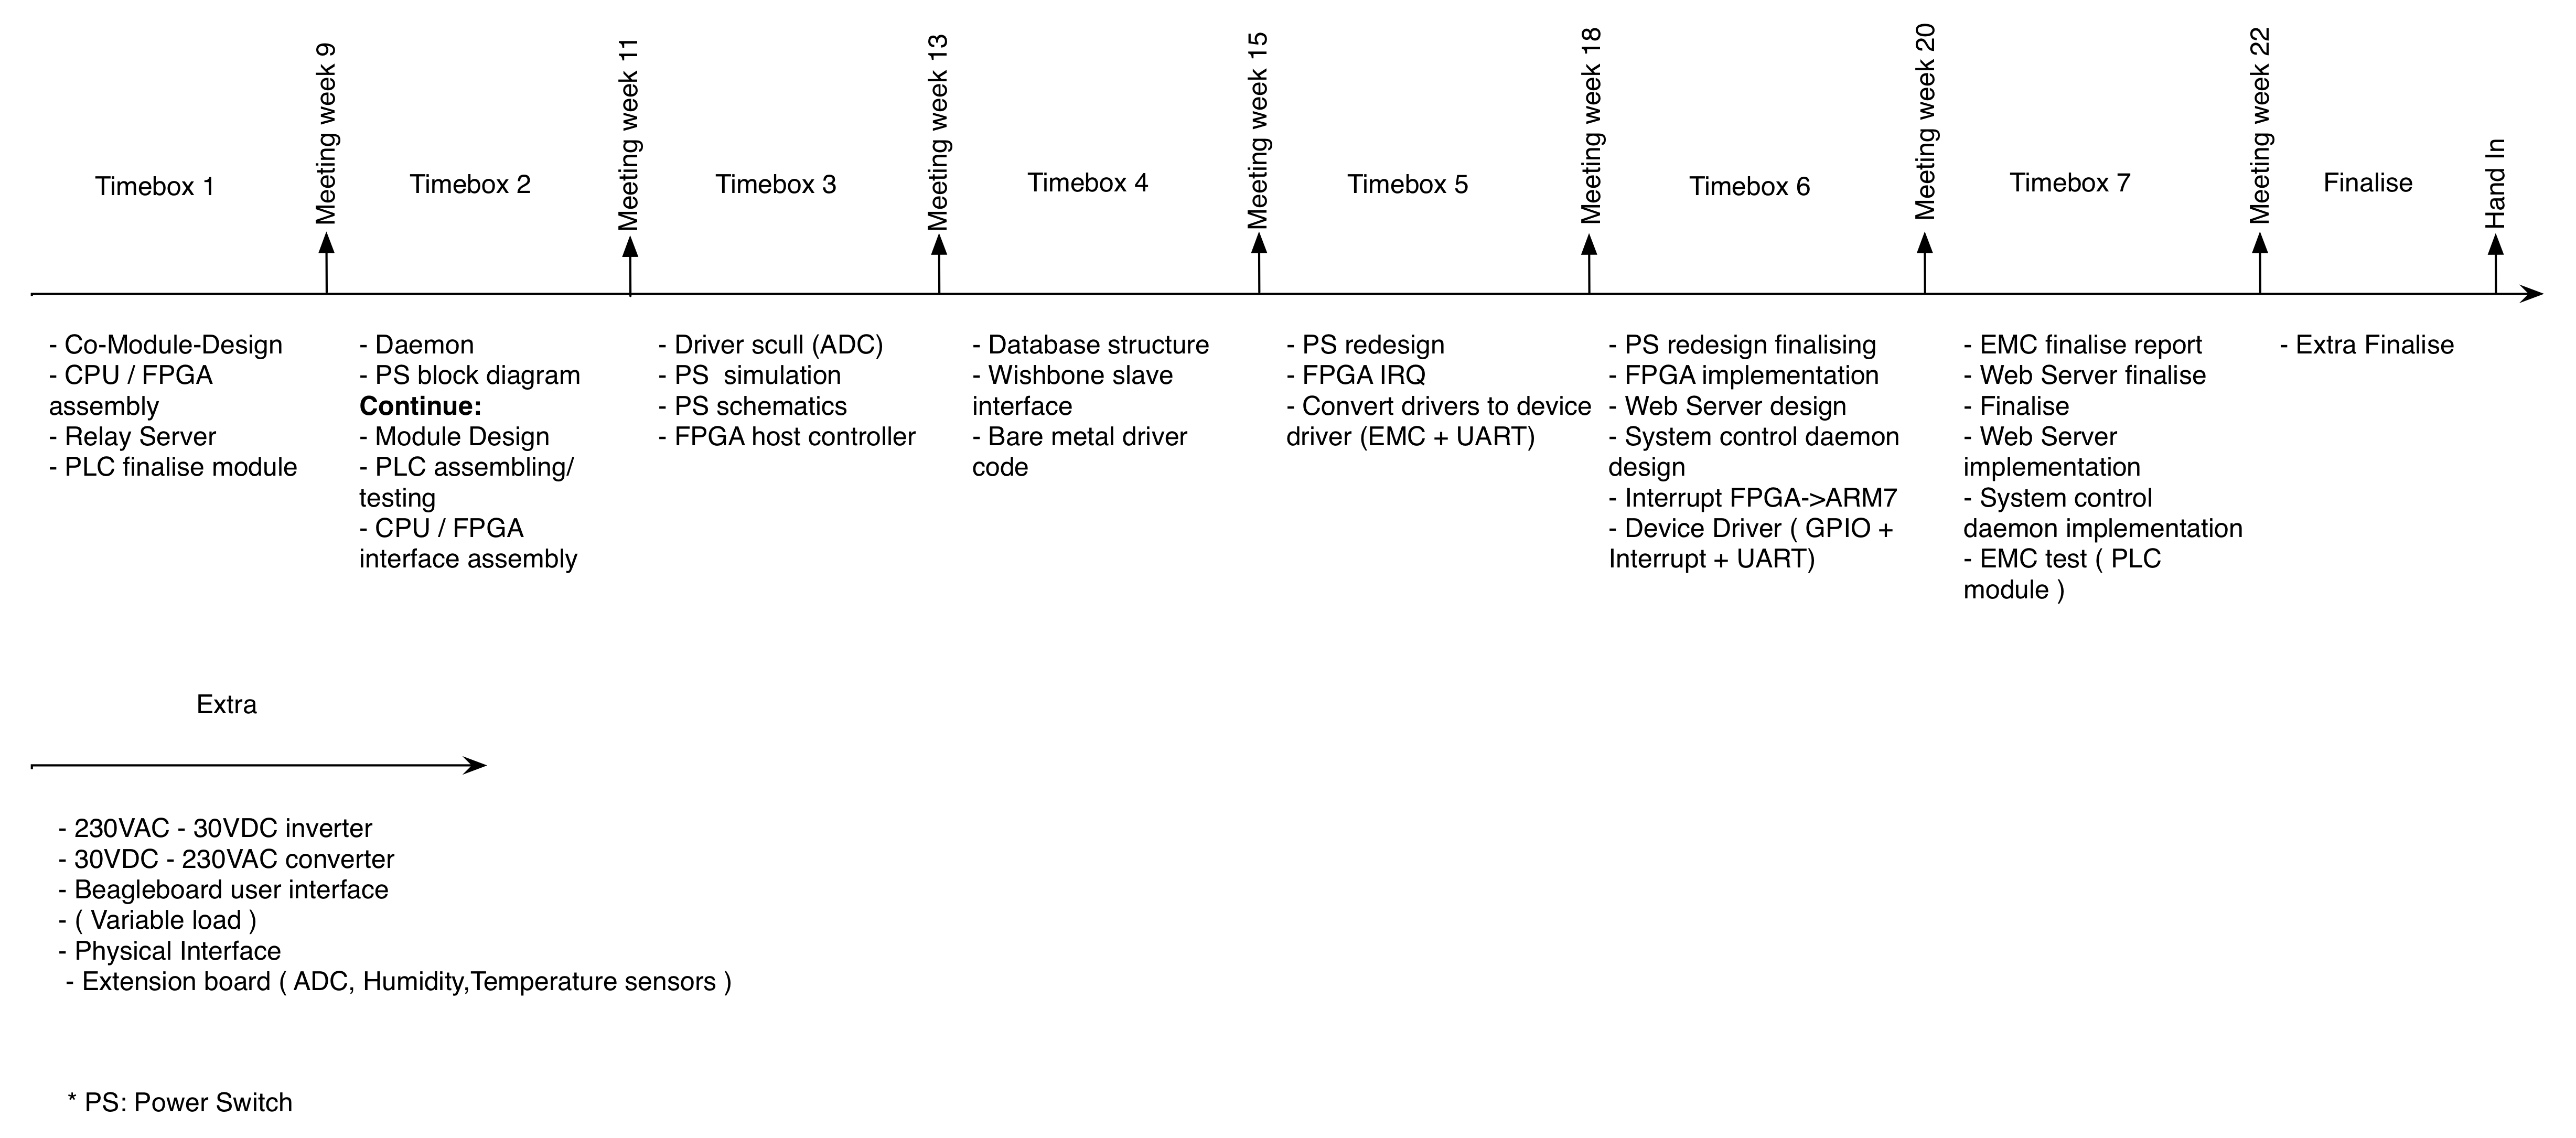
\includegraphics[width=1.0\textwidth]{images/tb_r5.png}
		%\caption{Updated time-box}
	\end{centering}
\end{figure}

\subsubsection{Work to be done in this time box}
\todo[inline]{Update List}
\begin{itemize}
	\item Requirements for debouncing
	\begin{itemize}
		\item Stability of switches
		\item Time limits
	\end{itemize}
	\item Verification
	\begin{itemize}
		\item External memory controller
		\item Verification of the Spartan 6
	\end{itemize}
	\item Jesus thing
		\begin{itemize}
			\item sub thing
		\end{itemize}
	\item Dennis thing
	\begin{itemize}
		\item Sub thing
	\end{itemize}
\end{itemize}

\paragraph{Description:}
\todo[inline]{Update Description}
\begin{description}
	\item[Requirements for debouncing] This is the timing requirements for the switch block to avoid bouncing when switching state
	\item[Verification] This is verification of the VHDL design including the EMC part in the LPC2478
	\item[Jesus thing]
	\item[Dennis thing]
\end{description}

\subsubsection{Time planning}

\begin{table}[H]
\centering
	\todo[inline]{Update Time}
	\begin{tabular}{|l|c|c|c|c|c|}
		\hline
		~			& Requirements for debouncing	& Verification			& Jesus thing		& Dennis thing	\\ \hline
		Estimation	& 3								& 7						& xx				& xx			\\
		Actual		& 3 							& xx					& xx				& xx			\\
		Developer	& Theis							& Theis					& Paulo				& Dennis		\\
		\hline
	\end{tabular}
	\caption{Estimation and actual time used on the project}
\end{table}
% % % % % % % % % % % % % % % % % % % % % % % % % % % % % % % % % % % % % % % % %
% % % % % % % % % % % % % % % % % % % % % % % % % % % % % % % % % % % % % % % % %
% Theis Thing
% % % % % % % % % % % % % % % % % % % % % % % % % % % % % % % % % % % % % % % % %
\subsection{Requirements for debouncing - Theis}
%			Intro
%					verification specification
%					deployment specification
%
This section is requirement update for the Switch block from section \ref{sec:Switch interrupt}.
\subsubsection{Analysis}
%			Analysis
%
%                Refactored block diagram
%                Refactored class diagram
%                Detailed use cases
%                User interface specification
%                System interface specification
%                Dimensioning specification 
%
In order to figure out how long the switches is bouncing, some measurement has been made on the switches, while it is shifted. The result is shown below.
\begin{figure}[H]
	\begin{centering}
		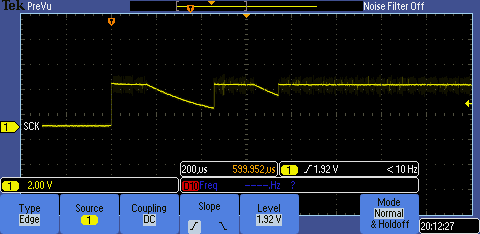
\includegraphics[width=0.7\textwidth]{images/debon_LtoH.png}
		\caption{Signal from switch. Low to high}
	\end{centering}
\end{figure}
From the figure above it is clear that the switch is bouncing, and it is possible to see how long it takes the switch to be stable. From the measurements it takes around $750\mu s$.
\begin{figure}[H]
	\begin{centering}
		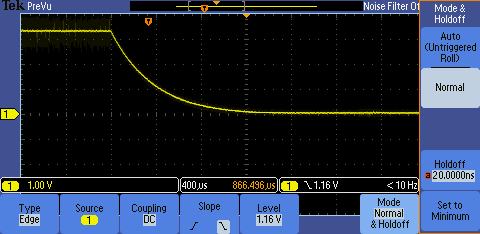
\includegraphics[width=0.7\textwidth]{images/debon_HtoL.png}
		\caption{Signal from switch. High to low}
	\end{centering}
\end{figure}
The figure above shows the switch signal from high to low, this signal is now bouncing, and would not cause any problem because the slope is negative at all time, so when the signal hits the point where the Spartan 6 is switching, the signal would not trigger a switch back. But is takes around $1200\mu s$ for the switch to stabilise.
\subsubsection{Design}
%       	 Design
%
%                UML/SysML deployment view(s)
%                Mechanical specifications and dimensioning
%                HW module specification per block
%                UML SW deployment view
%                Class specification
%                Refactored class diagram
%                Use case scenarios specifications
%                Sequence diagrams
%
In order to remove any debouncing on the switches, a delay is needed. In this system the time has to be the double plus one bit. From the measurements the longest time is $1200\mu s$, the double of that is $2400\mu s$. Calculations for the delay is shown below.
\begin{align}
	t &=	1200\mu s \cdot 2 \\
	f &=	100MHz\\
	t &=	2^{n}\cdot \dfrac{1}{f}\\
	n &=	\dfrac{\ln(f\cdot t)}{\ln(2)}\\
	n &=	\dfrac{\ln(100MHz\cdot 2400\mu s)}{\ln(2)}\\
	n &=	17.87
\end{align}
The bit length for the double delay is 18 and plus 1 bit, a 19 bit vector has to be used in the delay. The delay for 19 bit vector is.
\begin{align}
	t &=	2^{19}\cdot \dfrac{1}{100MHz}\\
	t &=	5.243 ms\\
\end{align}
This is the time delay that is used to debounce the switches.
\subsubsection{Conclusion}
This time delay has been tested in timebox 6 and it is working with the interrupt register in the Spartan 6.
%
%
%
% % % % % % % % % % % % % % % % % % % % % % % % % % % % % % % % % % % % % % % % %
\subsection{Verification - Theis}
%			Intro
%					verification specification
%					deployment specification
%
From the former timeboxes the blocks in the Spartan 6 has been implemented to make a complete system, which is communicating with the external memory controller in the LPC2478.
\subsubsection{External memory controller}
\begin{figure}[H]
	\begin{centering}
		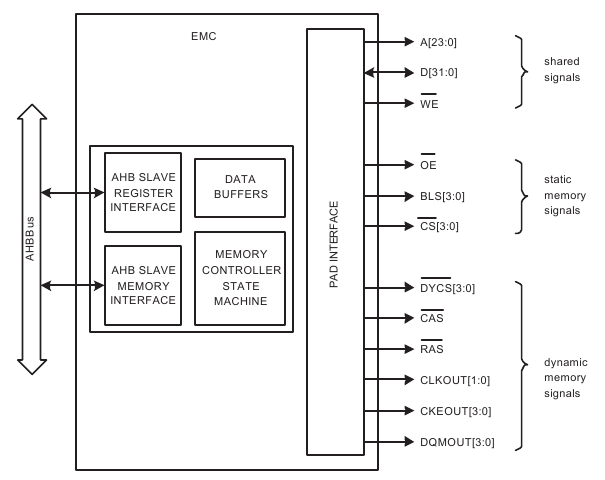
\includegraphics[width=0.8\textwidth]{images/tb7_EMC_block.png}
		\caption{EMC block}
	\end{centering}
\end{figure}
\begin{figure}[H]
	\begin{centering}
		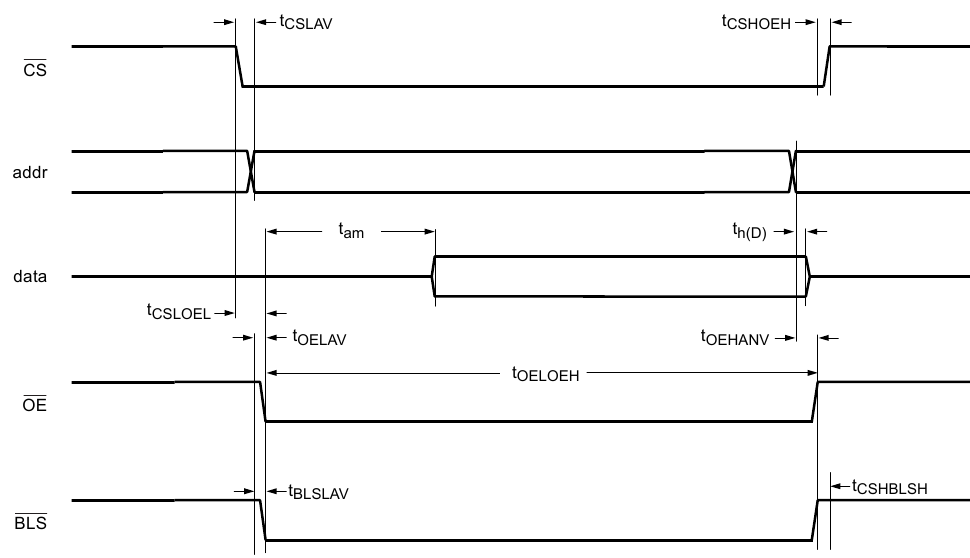
\includegraphics[width=0.8\textwidth]{images/tb7_EMC_read.png}
		\caption{EMC Read timing}
	\end{centering}
\end{figure}
\begin{figure}[H]
	\begin{centering}
		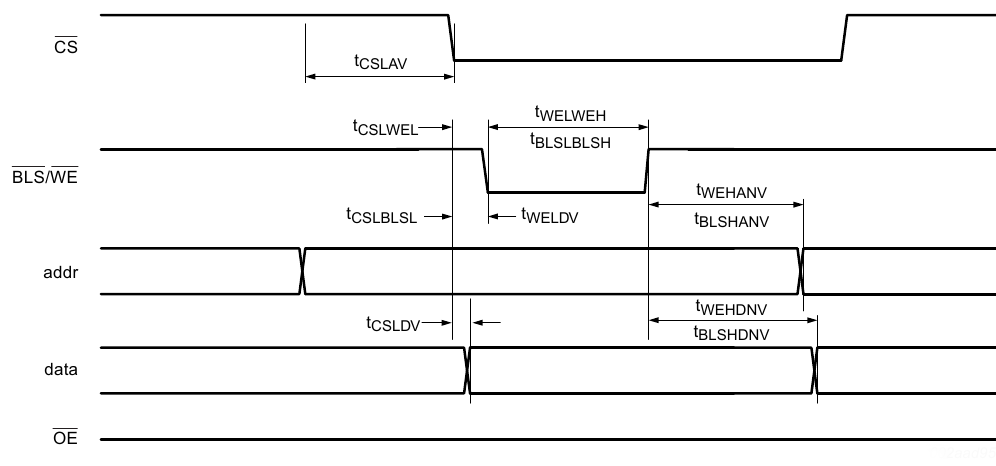
\includegraphics[width=0.8\textwidth]{images/tb7_EMC_write.png}
		\caption{EMC Write timing}
	\end{centering}
\end{figure}
\subsubsection{Bus functional module}
\begin{figure}[H]
	\begin{centering}
		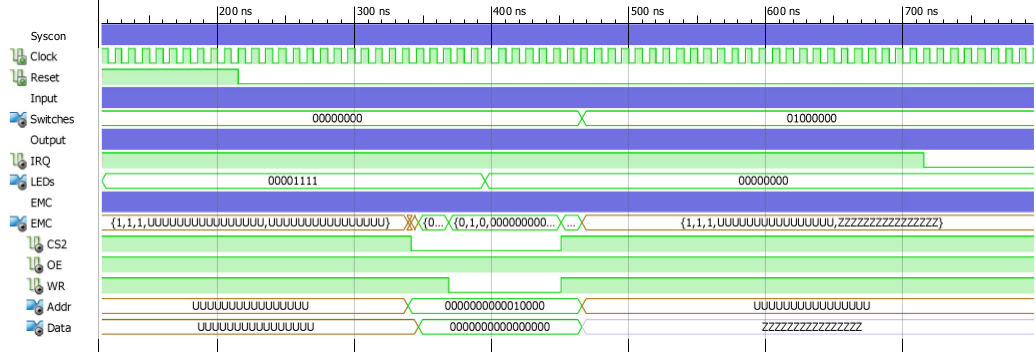
\includegraphics[width=1.0\textwidth]{images/tb7_BFM_write.png}
		\caption{BFM write}
	\end{centering}
\end{figure}
\begin{figure}[H]
	\begin{centering}
		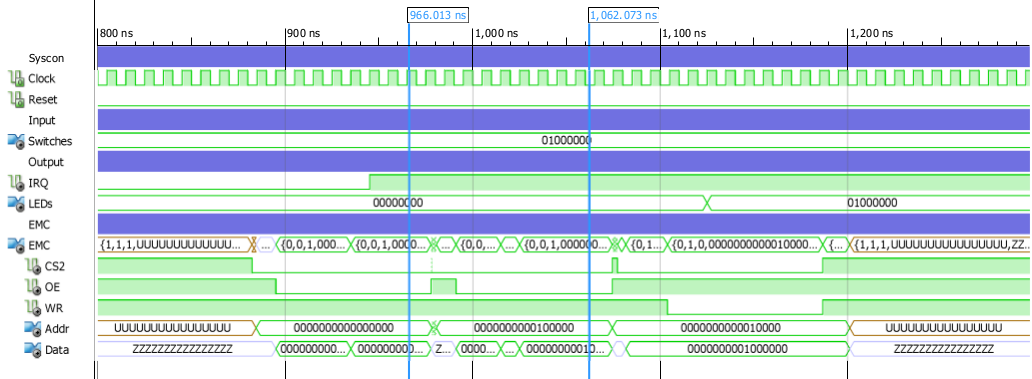
\includegraphics[width=1.0\textwidth]{images/tb7_BFM_read_irq.png}
		\caption{BFM read IRQ}
	\end{centering}
\end{figure}
\subsubsection{Spartan 6}

\begin{figure}[H]
	\begin{centering}
		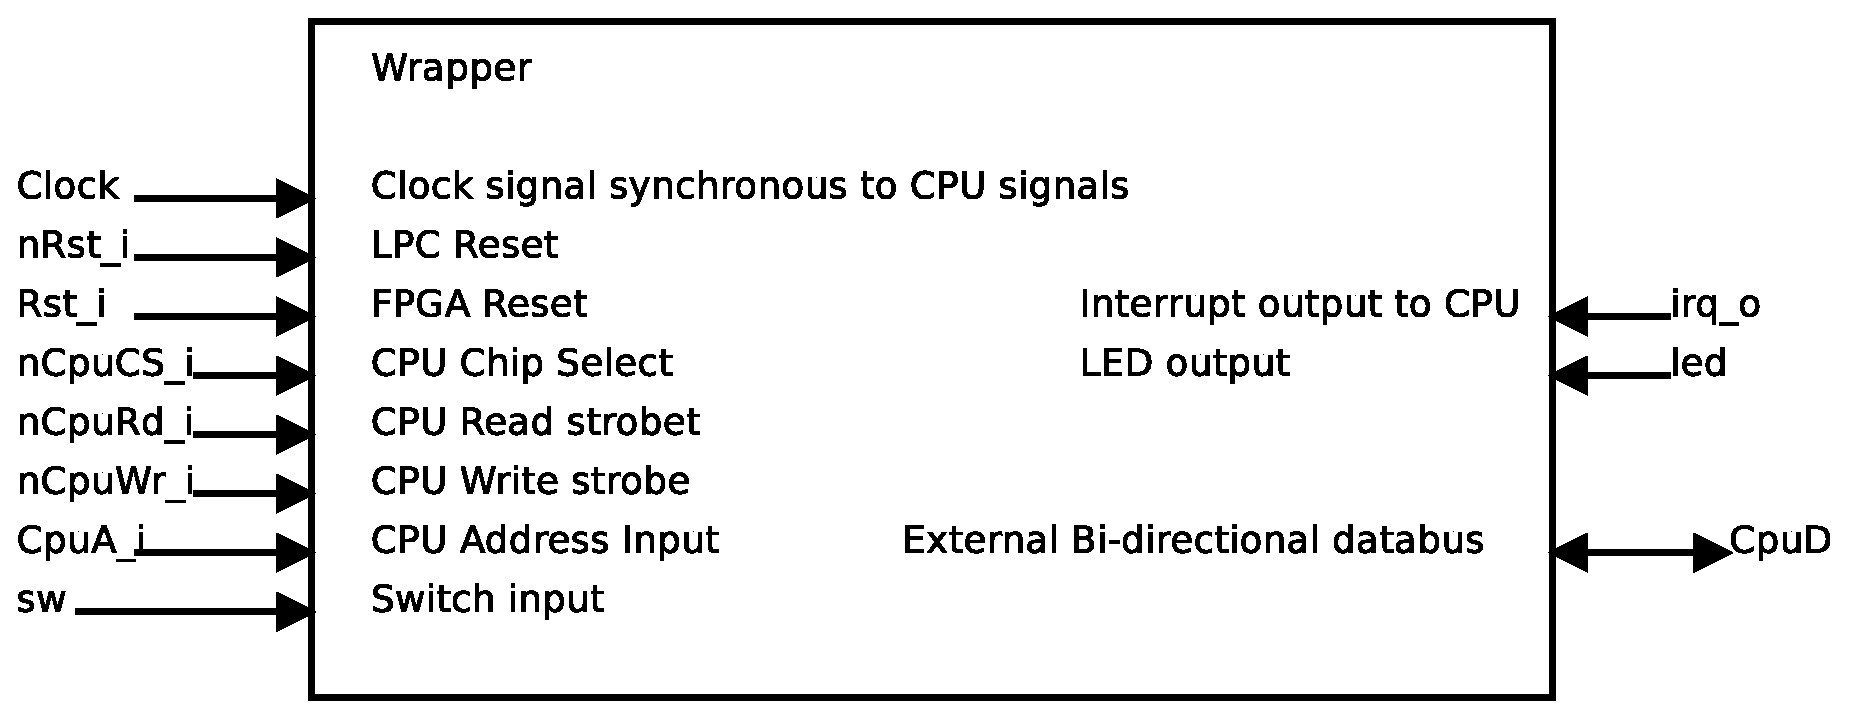
\includegraphics[width=0.9\textwidth]{images/tb7_wrapperblock.eps}
		\caption{Top level in Spartan 6}
	\end{centering}
\end{figure}

\begin{table}[H]
    \begin{tabular}{|l|l|l|l|l|l|p{3.7cm}|}
        \hline
        Name         & DIR		 & S select 	& S address 	& Data                & EMC address & Note                                  \\ \hline
        IRQ Register & Read      & 000          & 0000          & 7 bit - 6 down to 0 & 0x82000000        & Hold data from the interrupting slave \\ \hline
        LED          & Write     & 001          & 0000          & 8 bit - 7 down to 0 & 0x82000020        & Set states of LEDs                    \\ \hline
        Switch       & Read      & 010          & 0000          & 8 bit - 7 down to 0 & 0x82000040        & Hold state of switches                \\
        \hline
    \end{tabular}
    \caption{Memory map of Spartan 6\\
    		 S = Slave, DIR = Direction}
\end{table}
\subsubsection{Conclusion}
% % % % % % % % % % % % % % % % % % % % % % % % % % % % % % % % % % % % % % % % %
% % % % % % % % % % % % % % % % % % % % % % % % % % % % % % % % % % % % % % % % %
% Jesus Thing
% % % % % % % % % % % % % % % % % % % % % % % % % % % % % % % % % % % % % % % % %
\subsection{Jesus thing - Paulo}
%			Intro
%					verification specification
%					deployment specification
%
\subsubsection{Analysis}
%			Analysis
%
%                Refactored block diagram
%                Refactored class diagram
%                Detailed use cases
%                User interface specification
%                System interface specification
%                Dimensioning specification 
%
\subsubsection{Design}
%       	 Design
%
%                UML/SysML deployment view(s)
%                Mechanical specifications and dimensioning
%                HW module specification per block
%                UML SW deployment view
%                Class specification
%                Refactored class diagram
%                Use case scenarios specifications
%                Sequence diagrams
%
\subsubsection{Implementation}
%     	   Implementation
%
%                Mechanical drawings with details explained
%                Electronic diagrams with details explained
%                Source code with details explained
%                Description of integration 
%
\subsubsection{Verification}
%       	 Verification
%
%                Module tests
%                Integration tests
%                Acceptance test
\subsubsection{Conclusion}
% % % % % % % % % % % % % % % % % % % % % % % % % % % % % % % % % % % % % % % % %
% % % % % % % % % % % % % % % % % % % % % % % % % % % % % % % % % % % % % % % % %
% Dennis Thing
% % % % % % % % % % % % % % % % % % % % % % % % % % % % % % % % % % % % % % % % %
\subsection{Dennis thing - Dennis}
%			Intro
%					verification specification
%					deployment specification
%
\subsubsection{Analysis}
%			Analysis
%
%                Refactored block diagram
%                Refactored class diagram
%                Detailed use cases
%                User interface specification
%                System interface specification
%                Dimensioning specification 
%
\subsubsection{Design}
%       	 Design
%
%                UML/SysML deployment view(s)
%                Mechanical specifications and dimensioning
%                HW module specification per block
%                UML SW deployment view
%                Class specification
%                Refactored class diagram
%                Use case scenarios specifications
%                Sequence diagrams
%
\subsubsection{Implementation}
%     	   Implementation
%
%                Mechanical drawings with details explained
%                Electronic diagrams with details explained
%                Source code with details explained
%                Description of integration 
%
\subsubsection{Verification}
%       	 Verification
%
%                Module tests
%                Integration tests
%                Acceptance test
\subsubsection{Conclusion}
% % % % % % % % % % % % % % % % % % % % % % % % % % % % % % % % % % % % % % % % %
% % % % % % % % % % % % % % % % % % % % % % % % % % % % % % % % % % % % % % % % %
% Deployment
% % % % % % % % % % % % % % % % % % % % % % % % % % % % % % % % % % % % % % % % %
\subsection{Deployment}
	%which versions of the prototype the customer will get
	%with what functionality.
\paragraph{Theis thing}
%
%
\paragraph{Jesus thing}
%
%
\paragraph{Dennis thing}
%
%